\documentclass[14pt]{extarticle}
\usepackage{graphicx}
\usepackage[T1]{fontenc} 
\usepackage[margin=1in]{geometry}

% Custom captions: 1 pav.
\usepackage{caption}
\captionsetup[figure]{labelformat=empty}
\renewcommand{\thefigure}{\arabic{figure} pav.}

% Turinys vietoj Contents
\renewcommand{\contentsname}{Turinys}

\begin{document}

% Titulinis
\begin{titlepage}
	\begin{center}
		
\includegraphics[width=5cm]{images/ktu_logo.png}

		\textbf{Kauno technologijos universitetas}

		Informatikos fakultetas

		\vspace{3cm}

		\textbf{Laboratorinis darbas Nr. 3}

		\vspace{0.5cm}
		P175B120 Paslaugų programavimas debesų kompiuterijoje

	\end{center}

	\begin{flushright}

		\vfill

		\textbf{Arnas Bradauskas}

		Studentas

		\vspace{0.2cm}

		\textbf{Doc. Vytautas Pilkauskas}

		Dėstytojas

	\end{flushright}

	\begin{center}
		Kaunas, 2024
	\end{center}

\end{titlepage}

% Turinys
\tableofcontents

\clearpage

\section{Pirma dalis}

\begin{figure}[!htbp]
	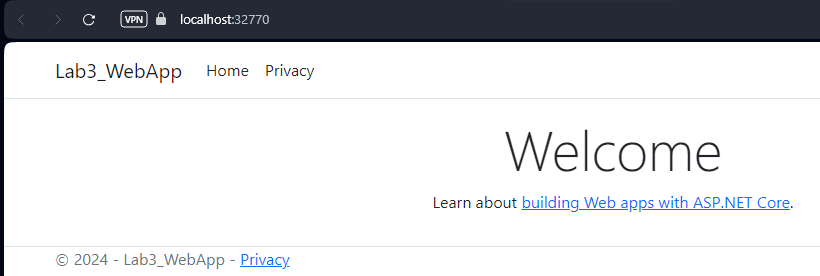
\includegraphics[width=\textwidth]{images/first/1.png}
	\caption{\thefigure\ Projektas paleistas lokaliai.}
\end{figure}

\begin{figure}[!htbp]
	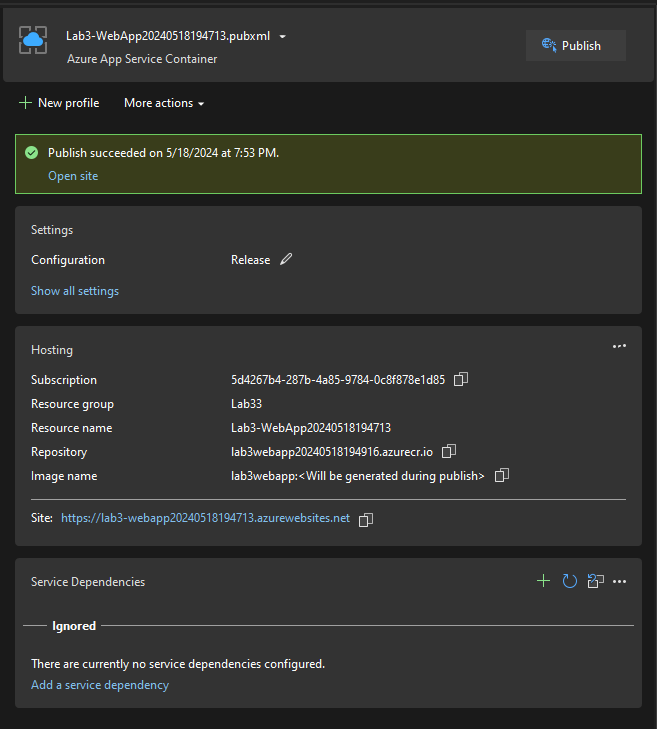
\includegraphics[width=\textwidth]{images/first/2.png}
	\caption{\thefigure\ Matomi rezultatai Visual Studio po Publish paspaudimo.}
\end{figure}

\begin{figure}[!htbp]
	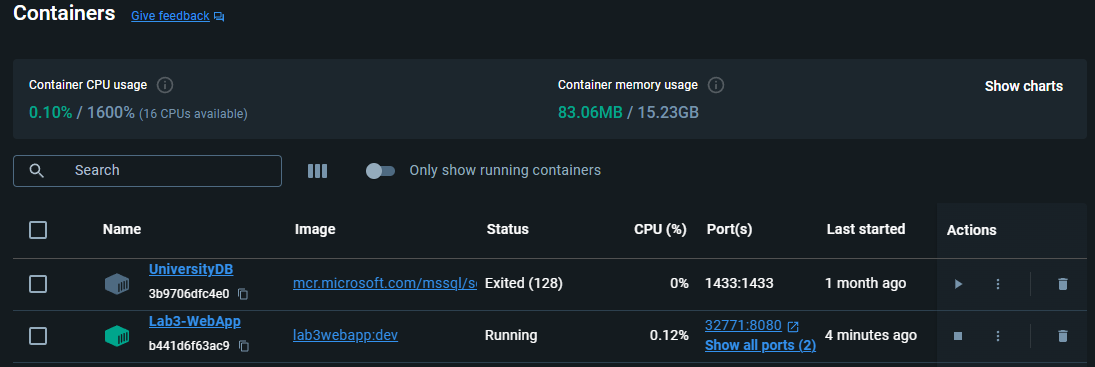
\includegraphics[width=\textwidth]{images/first/3.png}
	\caption{\thefigure\ Docker Desktop vaizdas.}
\end{figure}

\begin{figure}[!htbp]
	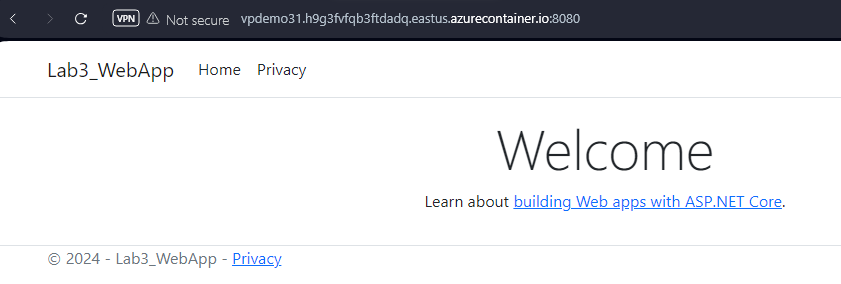
\includegraphics[width=\textwidth]{images/first/4.png}
	\caption{\thefigure\ Projektas paleistas Azure Container Instance.}
\end{figure}

\clearpage

\section{Antra dalis}

\begin{figure}[!htbp]
	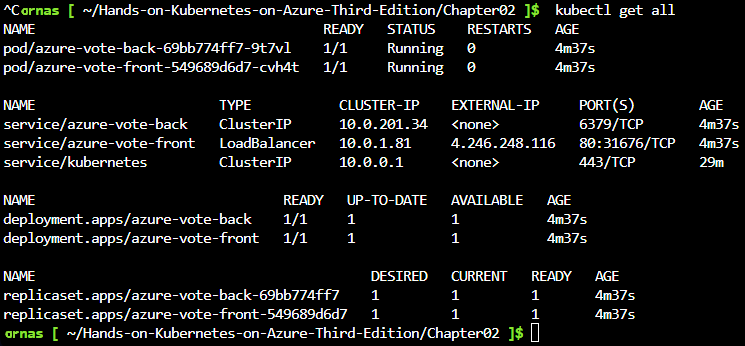
\includegraphics[width=\textwidth]{images/second/1.png}
	\caption{\thefigure\ Vaizdas po komandos `kubectl get all` mūsų klasteryje.}
\end{figure}

\begin{figure}[!htbp]
	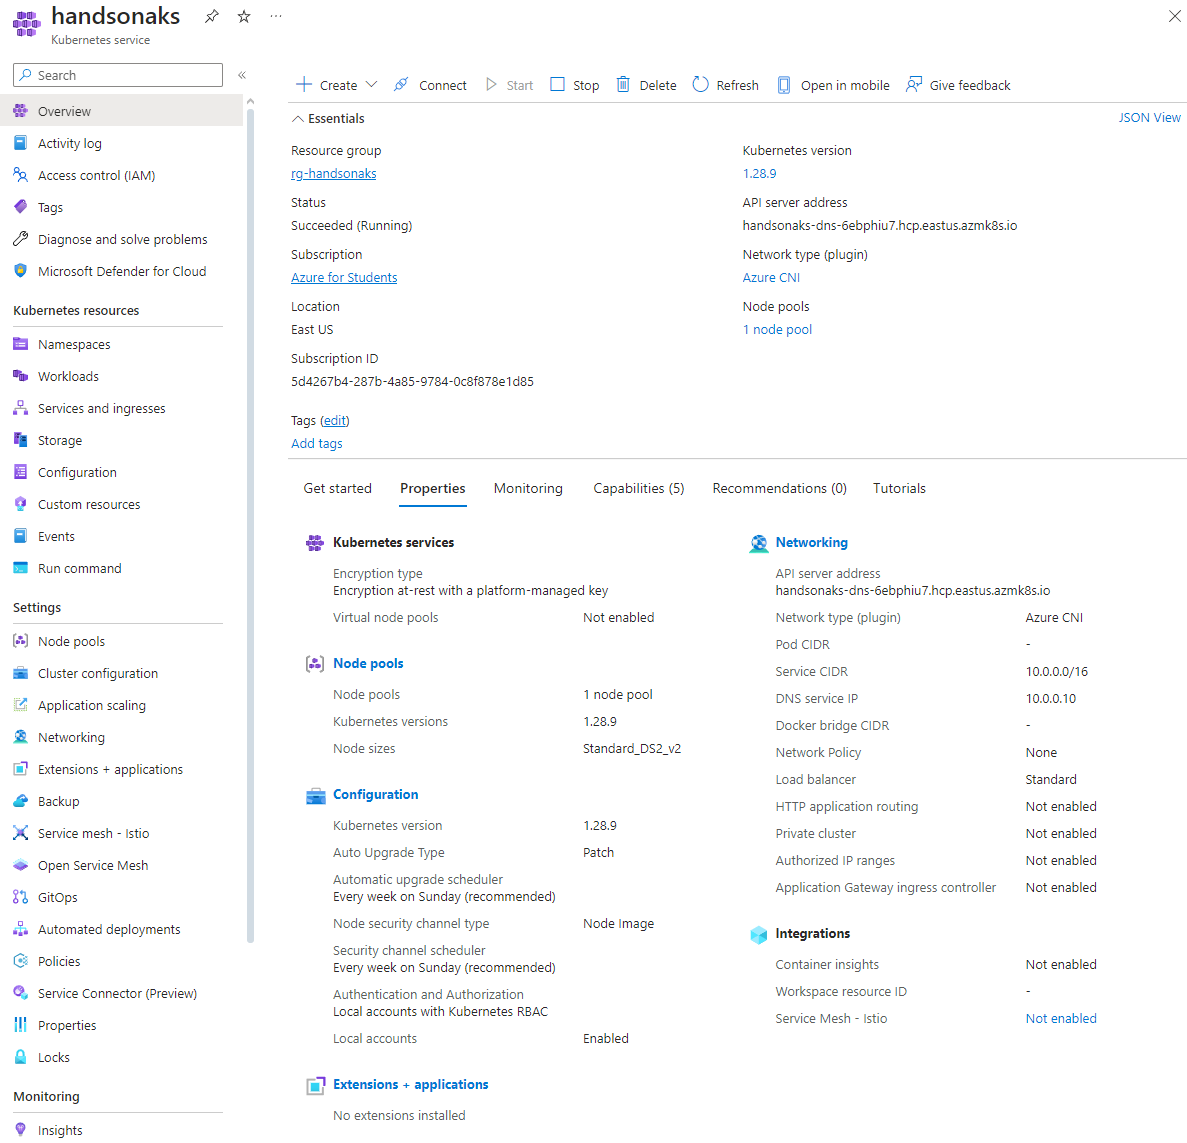
\includegraphics[width=\textwidth]{images/second/2.png}
	\caption{\thefigure\ Kubernetes klasterio Overview.}
\end{figure}

\begin{figure}[!htbp]
	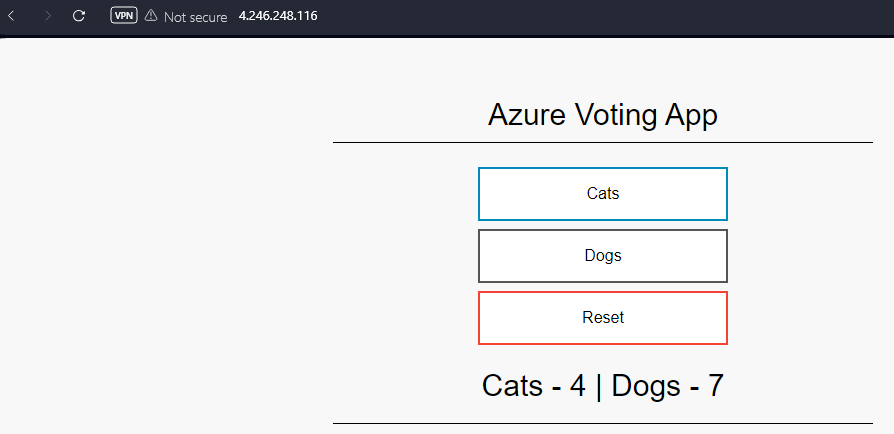
\includegraphics[width=\textwidth]{images/second/3.png}
	\caption{\thefigure\ Paleistas projektas klasteryje.}
\end{figure}

\clearpage

\end{document}
